%# -*- coding:utf-8 -*-
\documentclass[12pt,a4paper]{article}

\usepackage{buaa_paper}
\usepackage{fix-cm}


\schoolname{北京航空航天大学中法工程师学院}
\title{硕士学位论文中期检查报告}
\papertitle{基于词表分解优化的循环神经网络语言模型的研究}
\specialty{工业工程}
\studentnumber{ZY1624134}
\researcharea{自然语言处理}
\advisor{荣文戈~~副教授}
\author{是黎彬}
\date{2018 年 5 月 2 号}

\begin{document}

\maketitle



\addcontentsline{toc}{section}{摘要}
\keywords{大词表问题;词表分解;循环神经网络语言模型;自然语言处理}
{Over-large Vocabulary;\ Vocabulary Factorization;\ RNN Language Model;\ Natural Language Processing}

\begin{abstract_ch}
语言模型在自然语言处理领域起着非常重要的作用,该性能的好坏直接影响例如机器翻译和语音识别等很多任务的发展。随着循环神经网络的提出以及应用于语言模型上,计算机对人类语言的建模更加精确,但是也带来模型训练和运行速度都下降。尤其是当文本数据的数量急剧增长,单词的词表会变得巨大,这直接导致计算消耗十分大,包括计算复杂度太高所引起的运行耗时以及模型参数量太大所引起的内存占用过于庞大。为了解决这些问题,历史上人们开发了很多技术与模型,这些方法可以被分为三类:基于采样的近似算法,基于词表分解的算法,基于字母级别的编码模型。这些方法在一定程度上能缓解那些问题,但各自仍然存在一些缺陷。

本文首先概述课题研究的工作计划,包括研究目标和研究内容;其次,将汇报从开题至中期阶段已经完成的工作内容,包括对前人相关研究的总结;然后,将探讨这些方法中的一些关键技术,以及分析其中的一些弊病和技术难点;最后,汇报下一阶段的工作计划。

\end{abstract_ch}
\newpage
\begin{abstract_en}
Language model is a fundamental component in the field of neural language processing; its performance has direct influence on many tasks, e.g., machine translation and automatic speech recognition. With the propose of Recurrent Neural Network (RNN) and its inclusion in language model, language modeling by computer becomes more accuracy, yet producing the in-efficiency in the model’s training and operating. Especially when the text corpus growths explosively, vocabulary will become so huge that it causes both high computational complexity, which make it time-consuming to train as well as to infer, and excessive model size, which means the huge memory footprint. To tackle these problems, many techniques and models have been developed, mainly categorized as: sampling-based approximation, character level-based models, and vocabulary factorization-based methods.

In this paper we first introduce the work plan of this research project, containing the goals and the contents of this research. Then, we will report the works that we have done from the beginning to now, containing the resume of the previous related researches. Afterwards, we discuss the key techniques involved in these works and analyze analyze the existing problems and difficulties. Finally, we will report the work plan of next stage.


\end{abstract_en}
\newpage
\tableofcontents
\newpage

\section{论文工作计划}
\label{sec:intro}

\subsection{论文研究目标}

近年来,互联网技术的快速发展,尤其是各大社交网络平台技术日趋完善,为人们营造了一个便于交流的世界。于是,在全球范围内互联网用户数量在不断增加,用户之间的交流、用户对互联网产品的评论以及各种信息的共享,这造成互联网上的数据爆炸式增长。其中,文本数据是用户信息传递的载体,如何从文本数据中自动挖掘有用的信息便成了一个各大互联网公司研究的热点。由此,对无标注的文本语言进行建模(Language Modeling, LM)就成了文本数据挖掘的一项非常重要的基础工作,很多文本挖掘应用场景,如信息检索 \cite{Jin:2002:TLM:564376.564386}、 机器翻译 \cite{DBLP:conf/naacl/BaltescuB15}、 语音识别 \cite{DBLP:conf/interspeech/SakSB14},都需要以语言模型为基本模块。因此,此研究课题是具有很强的实用价值和研究意义的。

自2006 年Hinton 提出深度学习(Deep Learning, DL)以来 \cite{hinton2006reducing},将深度学习应用于自然语言处理(Natural Language Processing, NLP)任务中已经成为自然语言处理界的趋势,尤其是在语言模型中的应用。研究者提出可以用神经网络(Neural Network, NN)对语言进行建模,包括前馈神经网络模型(Feed-Forward Neural Network, FFNN)\cite{DBLP:conf/nips/BengioDV00} 和循环神经网络模型(Recurrent Neural Network, RNN)\cite{DBLP:conf/interspeech/MikolovKBCK10}。其中,RNN 由于其特殊的网络结构能够将当前词的历史信息存储起来,并作为当前词预测的依据。该结构克服了N-gram语言模型无法利用距离当前词较远的词的信息。此外,在RNN 对一个词序列进行建模时,离散的词被映射到连续稠密的词嵌入(Word Embedding)空间,在这低维空间进行计算学习词序列的特征来学习词与词之间的依赖关系。因此,循环神经网络语言模型(Recurrent Neural Network Language Model, RNNLM)在模型困惑度(Perplexity, PPL)和词识别率上都取得了最好的结果 \cite{DBLP:conf/icassp/MikolovKBCK11}。

尽管RNNLM已经取得了重大的成功,但该模型仍然存在着很多难点,其中一个最为显著的问题是词表过大(Over-large vocabulary)的问题 \cite{DBLP:conf/interspeech/ChenWLGW14}。对此,由于语言模型旨在学习人类语言的模式,那么这意味着用于训练模型的人类语料越大,那么语言模型越能拟合语言模式并能因此模型生成的文本更像人说的语句一样。于是为了让模型更好的学习,这就不可避免的使得语料库数据量不断增长。词表过大的问题将会对RNNLM造成两个方面的巨大挑战:1)高计算复杂度(Computational complexity) \cite{DBLP:conf/acl/ChenGA16};2)庞大的模型参数量(Model size) \cite{DBLP:conf/nips/LiQYHL16}。

为了强调这些挑战的严峻性,在此列举一个例子来对此进行分析。One Billion Words (OBW)数据集是一个近年来公开的训练语言模型的语料数据集,它包含约80万个不同的词,是一个典型的能够测试模型能否胜任词表过大这个问题的数据集。如果我们考虑一个标准的RNNLM,其中词嵌入向量的维度和RNN中的隐层的维度都设置为1024,并且在计算机中用32位浮点数去储存这些数据,那么通过计算可知该模型的大小达到7GB。 如此巨大的模型对于当前12GB 的图形处理元件(Graphics Processing Units, GPUs)是极其困难的,甚至当训练时候增大每一批次的数据量,该GPUs已经无法处理该模型了。此外,通过一些基础实验发现,该模型的训练非常耗时,甚至要花费1个月的时间才能训练好。由此可见词表过大对于RNNLM 是一个巨大的且亟待解决的问题。因此探讨研究语言模型的大词表问题,是目前理论应用到实际过程中必须要克服的问题,也是值得研究和探讨的问题。

本课题的研究目标就是针对在大数据背景下的词表过大的问题,研究该问题的症结所在,以及尝试提升目前的算法来缓解词表过大所带来的严重问题。

\subsection{论文主要研究内容}

\begin{itemize}
  \item 调研语言模型的相关背景与基础知识,了解在基于统计的语言模型方法过时之后,目前主流的基于深度学习的语言建模方法——循环神经网络语言模型。
  \item 深入探究循环神经网络语言模型,包括其理论知识以及代码实现,并从初步的实验中发掘“大词表”问题的根源所在。
  \item 考察目前存在的前沿的方法是如何解决语言模型中“大词表”问题的,包括基于采样技术,基于字符级别编码和基于词表分解三大类方法,本课题将重点探讨基于词表分解这一类方法。
  \item 深入探究基于词表分解的循环神经网络语言模型,包括基于预测层词表分解的方法和输入层词表分解的方法这两种,总结目前这一类方法存在的问题,并探索对其提升的性能的方法。
  \item 针对基于词表分解的循环神经网络语言模型,如何将词表进行分解是一个值得讨论与研究的问题,包括对词表的初始化分解方法,以及在建模过程中动态调整词表分布的方法。
\end{itemize}




\section{已经完成的工作}

\subsection{语言模型}
\subsubsection{基于统计的语言模型}
语言模型可以对一段文本的概率进行估计,对信息检索 \cite{Jin:2002:TLM:564376.564386}、 机器翻译 \cite{DBLP:conf/naacl/BaltescuB15}、 语音识别 \cite{DBLP:conf/interspeech/SakSB14} 等任务有着重要的作用。
形式化讲,统计语言模型的作用是为一个长度为$m$ 的字符串确定一个概率分布 $P(w_1;w_2;\cdots;w_m)$ ,表示其存在的可能性,其中$w_1$ 到$w_m$ 依次表示这段文本中的各个词。一般在实际求解过程中,通常采用下式计算其概率值:
\begin{equation}
\label{equ:lm}
\begin{split}
P(w_1;w_2; \cdots;w_m) &= P(w_1) P(w_2|w_1) P(w_3|w_1;w_2)\cdots P(w_i | w_1;w_2;\cdots;w_{i-1}) \\
&\cdots P(w_m | w_1;w_2;\cdots;w_{m-1})
\end{split}
\end{equation}
在实践中,如果文本的长度较长,公式 \ref{equ:lm} 右部$\cdots P(w_m | w_1;w_2;\cdots;w_{m-1}) $  的估算会非常困难, 因为出现$w_1;w_2;\cdots;w_{m-1};w_{m}$ 的语段非常少,进而该模型的稀疏性特别严重。因此,研究者们提出使用一个简化模型:n 元模型(n-gram model)。在n 元模型中估算条件概率时,距离大于等于n 的上文词会被忽略,也就是对上述条件概率做了以下近似:
\begin{equation}
\label{equ:approx}
P(w_i | w_1;w_2;\cdots;w_{i-1})  \approx P(w_i | w_{i-(n-1)};\cdots;w_{i-1})
\end{equation}
当$n = 1$ 时又称一元模型(unigram model),公式\ref{equ:approx} 右部会退化成$P(w_i)$,此时,整个句子的概率为:
\begin{equation}
P(w_1;w_2; \cdots;wm) = P(w_1)P(w_2) \cdots P(w_m)
\end{equation}
从式中可以知道,一元语言模型中,文本的概率为其中各词概率的乘积。也就是说,模型假设了各个词之间都是相互独立的,文本中的词序信息完全丢失。因此,该模型虽然估算方便,但性能有限。

当n = 2 时又称二元模型(bigram model),将n 代入公式\ref{equ:approx} 中,右部为P$(w_i|w_{i-1})$。 常用的还有n = 3 时的三元模型(trigram model),使用$P(w_i |w_{i-2};w_{i-1})$ 作为近似。这些方法均可以保留一定的词序信息 \cite{DBLP:journals/csl/ChenG99}。

\subsubsection{基于循环神经网络语言模型}
\label{sec:rnnlm}
Mikolov等人提出的循环神经网络语言模型(Recurrent Neural Network based Language Model,RNNLM)则直接对$P(w_i | w_1;w_2;\cdots;w_{i-1}) $ 进行建模,而不使用公式 \ref{equ:approx} 对其进行简化\cite{mikolov2012statistical,DBLP:conf/interspeech/MikolovKBCK10} 。因此,RNNLM 可以利用所有的上文信息,预测下一个词,其模型结构如图 \ref{fig:rnnlm} 所示。

\begin{figure}
  \centering
  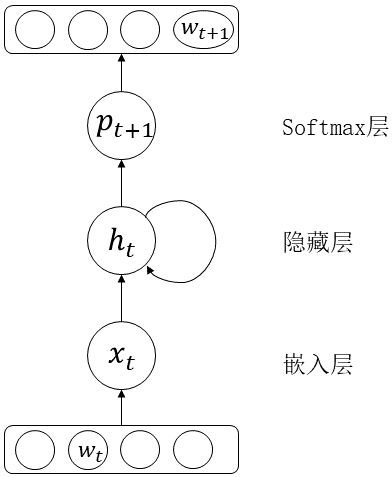
\includegraphics[width=0.85\linewidth]{./figures/rnnlm.png}
  \caption{循环神经网络语言模型(RNNLM)模型结构图}\label{fig:rnnlm}
\end{figure}

RNNLM 的核心在于其隐藏层的算法:
\begin{equation}
\label{equ:rnn}
h(i) =\phi(e(w_i) +Wh(i -1))
\end{equation}
其中,$\phi$非线性激活函数。但与NNLM 不同,RNNLM 并不采用n 元近似,而是使用迭代的方式直接对所有上文进行建模。在公式\ref{equ:rnn} 中,h(i) 表示文本中第$i$ 个词$w_i$ 所对应的隐藏层,该隐藏层由当前词的词向量$e(w_i)$ 以及上一个词对应的隐藏层$h(i -1)$ 结合得到。

隐藏层的初始状态为$h(0)$,随着模型逐个读入语料中的词$w_1;w_2; \cdots $, 隐藏层不断地更新为$h(1);h(2); \cdots$ 。根据公式\ref{equ:rnn},每一个隐藏层包含了当前词的信息以及上一个隐藏层的信息。通过这种迭代推进的方式,每个隐藏层实际上包含了此前所有上文的信息,相比NNLM 只能采用上文n 元短语作为近似,RNNLM 包含了更丰富的上文信息,也有潜力达到更好的效果。RNNLM 的输出层计算方法与NNLM 的输出层一致。


\subsection{大词表问题分析}
\label{sec:vocab}
本文已经在第\ref{sec:intro}章节通过举例凸显出词表过大的问题,此小节简单解释为什么词表过大会造成灾难性的问题。第\ref{sec:rnnlm}节已经详细地介绍了循环神经网络语言模型的(Recurrent Neural Network Language Model, RNNLM)的结果与原理,由此可知其建模过程为,RNNLM 使用一个嵌入层(Embedding Layer)将词映射至一个用稠密向量空间的表示词嵌入(Word Embedding),紧接着使用一个隐层(Hidden Layer)来对这些词嵌入进行编码,最后使用归一化指数函数(Softmax)进行预测下一个词在词表中的位置。

在这个过程中,词表的大小与Embedding Layer直接相关,因为所有在词表中的词都要通过Embedding Layer来获取向量表示才能进行后续的计算。我们可以简单的计算一下就可以发现其中的问题,假设一个数据集上的词表为$\mathcal{V}$,那么这个词表大小可以表示为${|\mathcal{V}|}$,另外不妨设词嵌入的向量维度为${|D|}$,那么这个Embedding Layer 的参数量为${\mathcal{O}(|\mathcal{V}| \times |D|)}$。当词嵌入维度${|D|}$不变,如果词表过大的话,那么这个参数量是十分巨大的,这是一个非常直观的影响。

同时,这个建模过程还直接影响Softmax,导致预测过程十分耗时。前面说过,Softmax 是用来依据当前词以及当前词的上下文的综合信息来预测下一个词的函数,这个预测也可以被看作是一个多分类(Multi-label Classification)任务。Softmax 预测的公式为如下:
\begin{equation}\label{eq:softmax}
\begin{split}
	p(w)=\frac{\exp(z_w)}{\sum_{w^{'}\in\mathcal{V}} {\exp(z_{w^{'}})}}
\end{split}
\end{equation}
其中$w$是指要在词表$\mathcal{V}$中预测的词,$z_w$指相关词的非归一化的激励分值。但是公式中的归一化项${Z=\sum_{w^{'}\in\mathcal{V}} {\exp(z_{w^{'}})}}$ 需要遍历整个词表上对所有词的预测分值进行求和,会带来非常高的计算量并使得模型低效。对于一个大小为${|\mathcal{V}|}$ 的词表,Softmax的计算复杂度等于${\mathcal{|\mathcal{V}|}}$,那么当词表过大的时候,该模块的计算量就会巨大。

为了尝试解决这些问题,很多种方法被开发出来,他们可以被分成3类:基于采样的近似,基于字符级别的建模以及基于词表分解的预测。以下章节对这三类方法一一介绍。

\subsection{基于采样近似方法}
由上一小节介绍可知,模型的计算复杂度很大程度上来源于Softmax中的归一化项,每一个词的预测都需要在整个词表范围内做求和计算,这个计算量必然庞大。针对这个问题,研究者们就发明了一些采样方法来对此做一些近似,这就是基于采样的近似方法(Sampling-based Approximation)。重要性采样(Importance Sampling, IS)\cite{DBLP:conf/aistats/BengioS03}、自适应重要性采样(Adaptive Importance Sampling, AIS)\cite{DBLP:journals/tnn/BengioS08}、噪声对比估计(Noise Contrastive Estimation)\cite{DBLP:journals/jmlr/GutmannH12,DBLP:conf/icml/MnihT12}以及负采样(Negative Sampling)\cite{DBLP:journals/corr/abs-1301-3781}都是属于这一类的方法。这些方法的核心思想是通过采样技术从词表中选取一部分的词来近似计算Softmax预测以及该函数的梯度。其中,最具代表性的且比较稳定的方法是NCE,下文对该方法做一个详细的介绍。
NCE是一种Mnih和Teh发明的比重要性采样更稳定的采样方法,该方法不是直接估计某个词的概率值,相反,它的学习目标是训练一个模型能够将正确的目标词和采样出来的噪声区分开。于是待解决的问题就由从词表中预测出正确的词语的复杂问题化简为一个二分类问题,即训练一个分类器尝试将正确的词语与所有其他噪声样本中的错误词区分出来,如图所示。
\begin{figure}
  \centering
  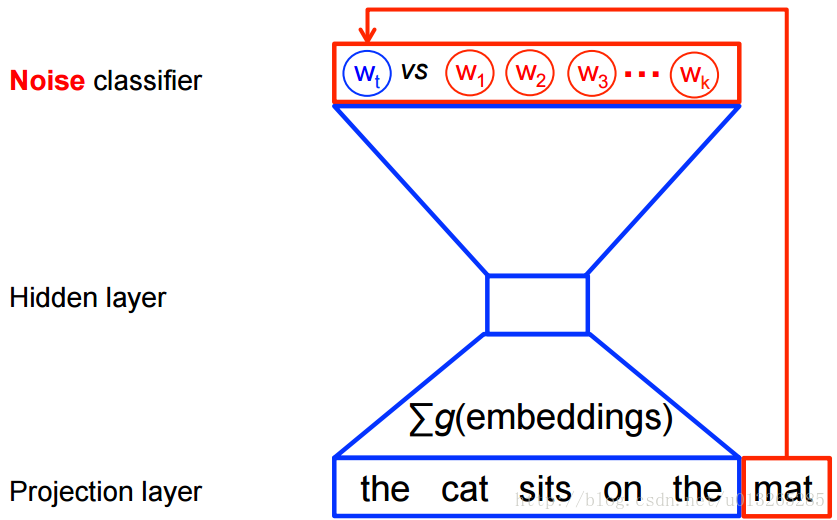
\includegraphics[width=0.6\linewidth]{./figures/nce.png}
  \caption{噪声对比估计(NCE)}\label{fig:nce}
\end{figure}

对于每个词${w_i}$,它的前n个词${w_{t-1},\cdots,w_{t-n+1}}$表示为语境${c_i}$。 然后从含有噪声分布$Q$中生成$k$个噪声样本${\tilde{w}_{ik}}$,由于是一个二分类问题,那么可以标记正确词$w_i$为正样本${(y=1)}$,标记剩下的噪声词${\tilde{w}_{ik}}$为负样本${(y=0)}$。

于是按二分类常用的代价函数来训练:
\begin{equation}
J_\theta = -\sum\limits_{w_i \in \mathcal{V}}{[\log P(y=1|w_i, c_i) + k\mathbb{E}_{\tilde{w}_{ik}}[\log P(y=0|\tilde{w}_{ik}, c_i)]]}
\end{equation}
其中$\mathbb{E}$表示期望,那么该公式可以简化为:
\begin{equation}
J_\theta = -\sum\limits_{w_i \in \mathcal{V}}{[\log P(y=1|w_i, c_i) + \sum\limits_{j=1}^k{\log P(y=0|\tilde{w}_{ik}, c_i)}]}
\end{equation}
剩下的是要推导出该公式中的概率值来:已知所有预测词都是从两个分布中采样得到的,其中正样本可以看做是从训练集${P_{train}}$中采样,而负样本是从噪声分布$Q$ 中采样得到,因此概率可以看做是两部分的按比组合为:
\begin{equation}
P(y,w|c) = \frac{1}{k+1} P_{train}(w|c) + \frac{k}{k+1}Q(w)
\end{equation}
于是,一个词来自训练集样本的概率为:
\begin{equation}
\begin{split}
P(y=1|w,c) &=  \frac{\frac{1}{k+1} P_{train}(w|c)}{\frac{1}{k+1} P_{train}(w|c) + \frac{k}{k+1}Q(w)} \\
           &= \frac{P_{train}(w|c)}{P_{train}(w|c) + kQ(w)} \\
           &= \frac{\frac{\exp(z_w)}{Z}}{\frac{\exp(z_w)}{Z} + kQ(w)}
\end{split}
\end{equation}
其中,$Z$为归一化项,也就是公式\ref{eq:softmax}里的归一化项。这一项的计算量非常大,而NCE 采用一个小技巧来避免,NCE的作者Mnih 和Teh把$Z$的值固定为1,他们认为这个近似对模型不会造成太大的影响。于是该公式就变为,
\begin{equation}
  P(y=1|w,c) = \frac{\exp(z_w)}{\exp(z_w) + kQ(w)}
\end{equation}
带入上述的代价函数中,最终得到NEC的代价函数:
\begin{equation}
J_\theta = -\sum\limits_{w_i \in \mathcal{V}}{\left[\log \frac{\exp(z_w)}{\exp(z_w) + kQ(w)} + \sum\limits_{j=1}^k{\log \frac{\exp(z_{\tilde{w}})}{\exp(z_{\tilde{w}}) + kQ(\tilde{w})}}\right]}
\end{equation}

NCE方法有完美的理论证明:随着噪声样本$k$的数量增加,NCE导数趋近于Softmax 函数的梯度。Mnih 和Teh 认为抽取25个噪声样本就足以到达Softmax函数的效果,而速度能提升大约45 倍,这是一个非常好的提升\cite{DBLP:conf/icml/MnihT12}。
\subsection{基于字符级别建模方法}
\begin{figure}
  \centering
  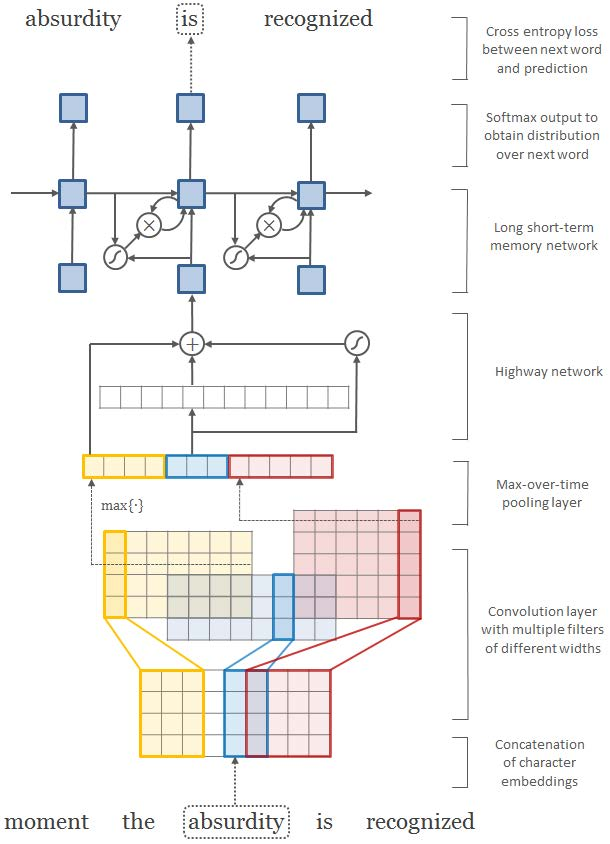
\includegraphics[width=0.4\linewidth]{./figures/CharCNN.jpg}
  \caption{基于字符级别建模的语言模型}\label{fig:charcnn}
\end{figure}
本文在第\ref{sec:vocab}章节分析了由词表过大带来的问题,那么就意识到需要针对这个大词表做一些处理。对此,Kim发明了CharCNN\cite{DBLP:conf/aaai/KimJSR16},与之前的方法在词级别建模的方法相比,该方法利用英语单词的特殊性——尽管词的数量非常庞大,但是所有词都由26个字母组成。如果能在对字母级别进行建模,那模型的大小能得到缩减。CharCNN就是用字符级别的输入代替原始的词级别的输入,那么这能将词嵌入层的参数从原始的${\mathcal{O}(|\mathcal{V}| \times |\mathcal{D}|)}$缩减至${\mathcal{O}(|Char| \times |\mathcal{D}|)}$,其中${|Char|}$指的是字符的数量。其完整的建模过程在图\ref{fig:charcnn}中列出。

尽管该方法能利用字符数量少的特性来将模型的大小缩减,但是仍然存在着一些问题,比如字符级别只能被用在嵌入层,而Softmax层的参数量没有变,因为它扔需在词表范围内去做预测,那么它还要遭受Softmax层在大词表上预测低效性的困扰。此外,这一方法只能应用于西方语言建模问题上,而对于中文字,这个方法就失效了。

\subsection{基于词表分解预测方法}
\label{sec:vocab_facto}

\subsubsection{Hierarchical Softmax}
\label{sec:hsm}

与前两类的方法不同的是,基于词表分解的方法是在词级别输入上进行建模的,而且该方法在预测的时候也没有近似。该类方法使用完整的词表,并且利用词表的结构性和层级性以及条件概率把原来的词的一步预测分解成多步预测问题。这一类的方法有很多,包括基于双层结构Softmax(Class-based Hierarchical Softmax, cHSM)的方法\cite{DBLP:conf/icassp/Goodman01,DBLP:conf/icassp/MikolovKBCK11,DBLP:conf/acl/ChenGA16,DBLP:conf/icml/GraveJCGJ17} 和基于树层级结构Softmax(Tree-based Hierarchical Softmax, tHSM)的方法\cite{DBLP:conf/aistats/MorinB05,DBLP:conf/nips/MnihH08}。

对于cHSM来说,他们的核心想法是要把通过传统的Softmax进行词的预测方法分裂成两个步骤。原来的Softmax 是直接把一个词从词表中预测出来,而cHSM是先预测这个词属于的类别,然后再在这个类别中预测出具体哪个词,公式可以表示为如下:
\begin{equation}
\label{eq:cHSM}
\begin{split}
	p(w|h)=p(c|h)p(w|c,h)
\end{split}
\end{equation}
其中$h$表示词$w$的上下文信息。如果我们把词表$\mathcal{V}$中的所有词分配到${\sqrt{|\mathcal{V}|}}$个平衡的类中(平衡意味着每个类里面的单词数量是一致的),那么该计算复杂度就由原来的${\mathcal{O}(|\mathcal{V}|)}$ 缩减到${\mathcal{O}(\sqrt{|\mathcal{V}|})}$。

cHSM从一开始由Goodman(2001)发明出来一直到现今仍然有相近的方法提出,其核心的加速原理一直没用变。从深度学习流行之前Goodman 用最大熵语言建模(Maximum Entropy Language Model)方式\cite{DBLP:conf/icassp/Goodman01}到目前流行的循环神经网络的建模方式\cite{DBLP:conf/asru/MikolovDPBC11};以及无论该方法中类的组织关系作何变化,包括层级组织结构\cite{DBLP:journals/jmlr/BengioDVJ03}、 并列组织结构\cite{DBLP:conf/icassp/MikolovKBCK11}和分片组织结构\cite{DBLP:conf/acl/ChenGA16},这三种组织结构的示意图如图\ref{fig:softmax} 所示。
\begin{itemize}
  \item 层级组织结构:该结构就是一个最经典的两层的层级Softmax,先预测词的类别,然后在该类别中预测词,如图\ref{fig:softmax}中(a)所示;
  \item 并列组织结构:该结构将词的类下标和类中词下标合并在一起,然和同时预测这两个下标,如图\ref{fig:softmax}中(b)所示;
  \item 分片组织结构:该结构认为文本中的词会根据词出现频率而具有不同的重要性,词频越大,那么该词就越重要。基于这个想法,该结构先根据词频大小将词表划分成多个片段,然后给每个片段赋予不同的参数量,如果片段词频大,那么就要赋予更多的参数去学习他们的特征。其结构如图\ref{fig:softmax} 中(c) 所示。
\end{itemize}
\begin{figure}
  \centering
  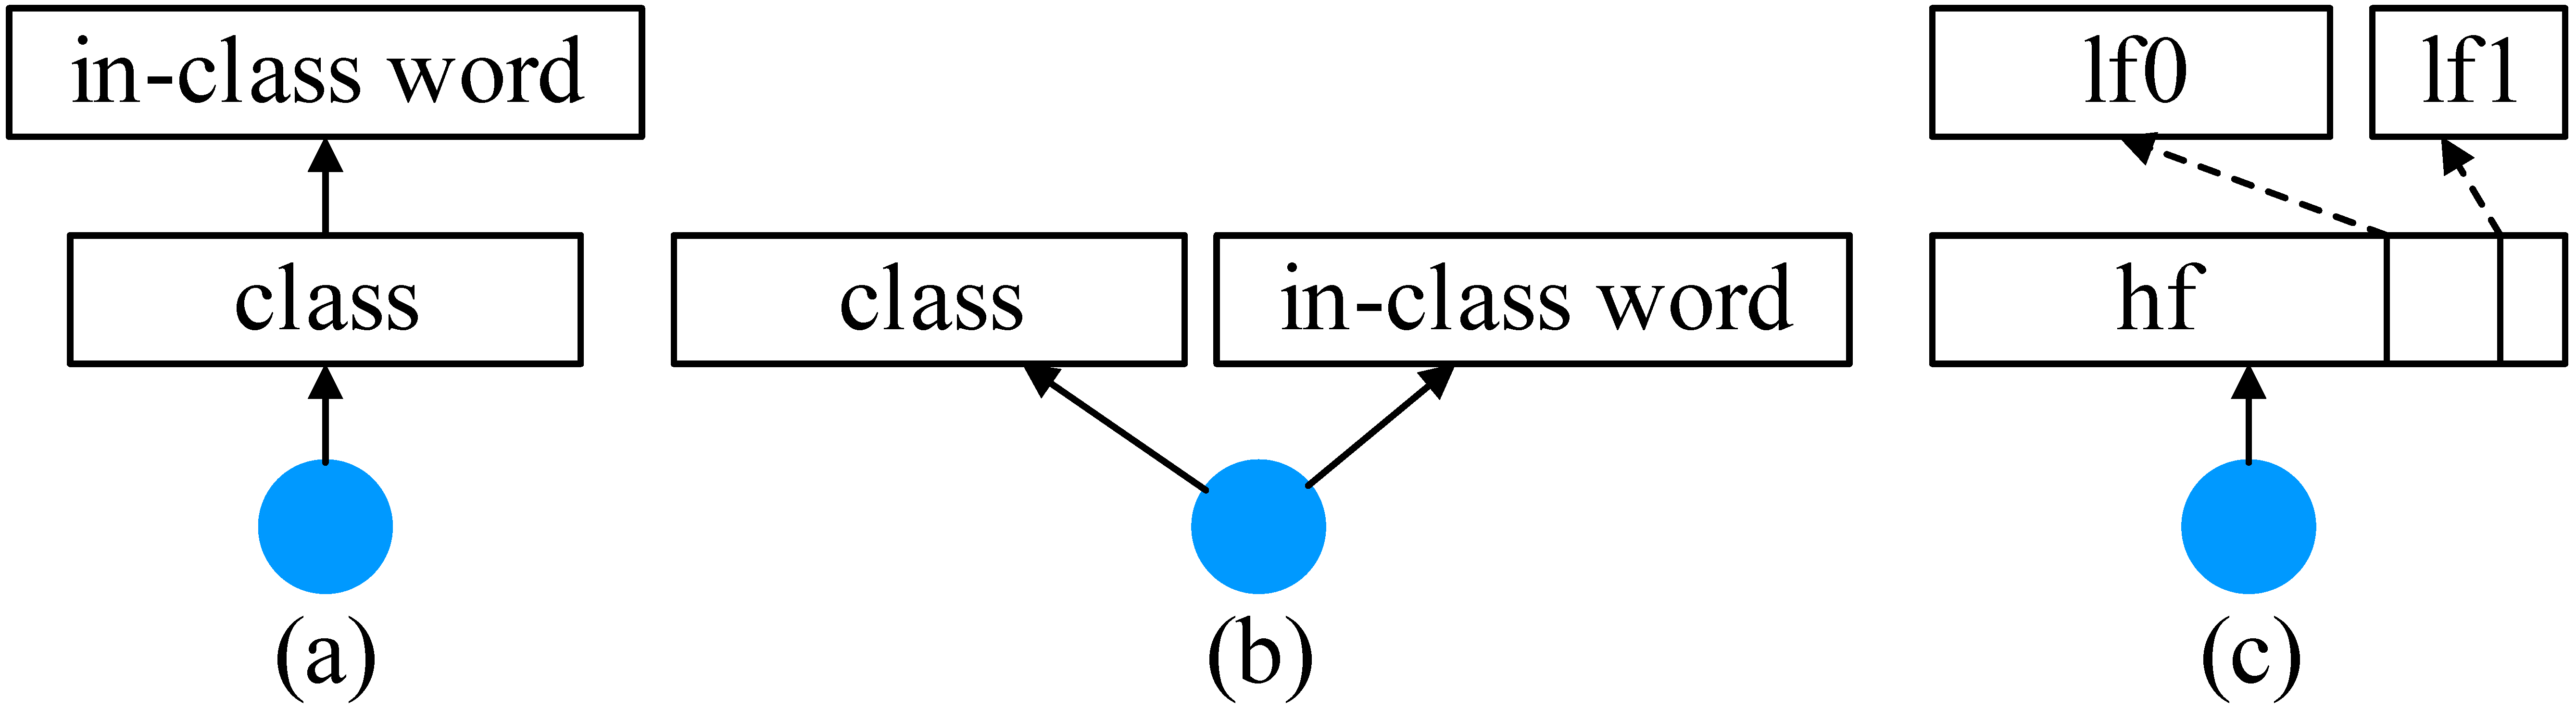
\includegraphics[width=0.65\columnwidth]{./figures/softmax3.png}
  \caption{三种不同的在Softmax层中词类组织关系的结构。(a) 层级组织结构;(b) 并列组织结构;(c) 分片组织结构,图中hf表示高频(high frequency),而lf表示低频(low frequency),其中lf0和lf1是根据词的低频程度把词分配起来。另外,在图中蓝色的单元表示包含历史信息和当前输入词信息的隐层,这一点对于这三种方法都一致。}
  \label{fig:softmax}
\end{figure}

对于tHSM,它可以被看作是cHSM的延伸。tHSM扩展了cHSM的思想,把Softmax层继续分裂,直到把原始的Softmax分裂成一个树结构(Tree)。所有的词都列在在这棵树的叶子节点(Leaf Node)上,而这棵树的中间节点表示词表的深层次结构,如图\ref{fig:thsm}所示。如果考虑用一个平衡的二叉树结构来组织词类的结构关系,那么这种tHSM的计算复杂度又继续减小至${\mathcal{O}(\log |\mathcal{V}|)}$。
\begin{figure}
  \centering
  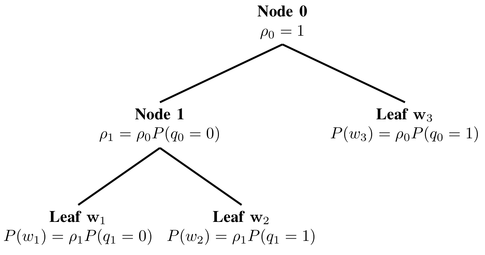
\includegraphics[width=0.65\columnwidth]{./figures/thsm.jpg}
  \caption{树结构层次Softmax}
  \label{fig:thsm}
\end{figure}

\subsubsection{LightRNN}

前面介绍的方法要么专门用来减小计算复杂度以加速,要么专门用来缩减模型的大小,却没有一个模型同时能在来两方面同时进行优化的。LightRNN方法的提出不仅能减小模型计算复杂度,还能大幅度缩减模型的大小\cite{DBLP:conf/nips/LiQYHL16}。基于该想法,LightRNN提出一个2-Component shared embedding,将词分配到一个二维的词表里面。词表所有相同行的词共享一个行向量,所有相同列的词共享一个列向量。而一个词由其对应的行向量与列向量联合表示。这样,我们就仅需要${2\sqrt{|\mathcal{V}|}}$个向量来表示词表中所有的词。对于每个用行标和列标表示的词来说,LightRNN更改了原始的RNN 结构来对双标表示的词进行编码,其结构如图\ref{fig:lightrnn}。这种方法能够将词嵌入层和Softmax层的维度降低至${\mathcal{O}(\sqrt{|\mathcal{V}|} \times |D|)}$ 和${\mathcal{O}(\sqrt{|\mathcal{V}|} \times |H|)}$。该方法的另一个值得学习的地方是将词交换问题变成一个最小费用最大流问题(Minimum Cost Maximum Flow, MCMF),并利用一个优化算法\cite{Preis1999}去解决这个问题。
\begin{figure}[!ht]
  \centering
  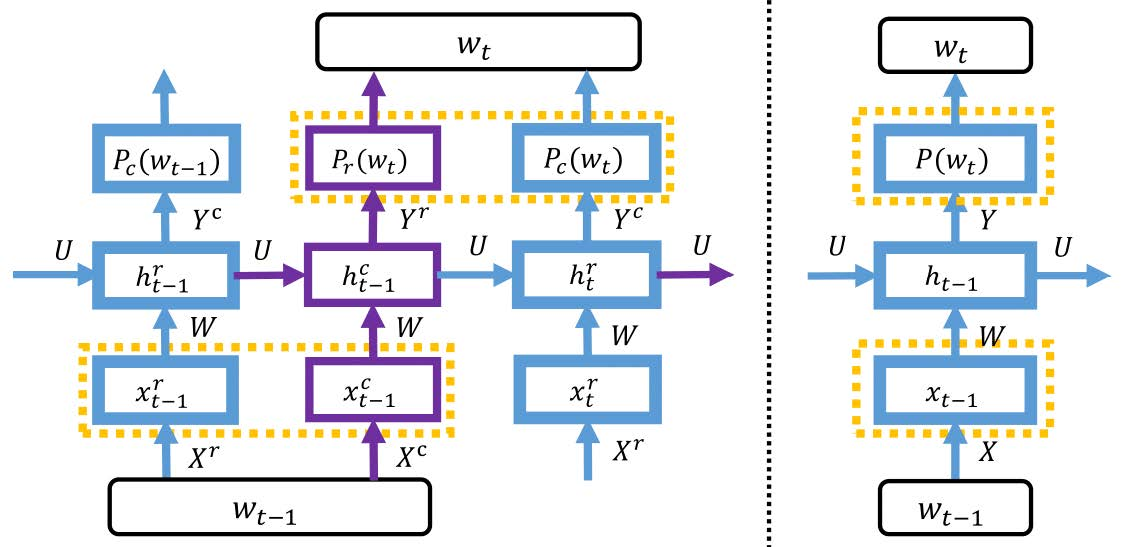
\includegraphics[width=0.65\columnwidth]{./figures/lightrnn.jpg}
  \caption{LightRNN}
  \label{fig:lightrnn}
\end{figure}

\section{关键技术和难点}

\subsection{循环神经网络及其变种}
随着深度学习(Deep Learning)的兴起,将深度学习模型应用于自然语言处理(Natural Language Processing)已经成为一大趋势,其中循环神经网络(Recurrent Neural Network, RNN)扮演着非常重要的角色。因为语言的基本构成是语句,而语句可以被看作是一个词序列,所以RNN利用其对序列数据建模的友好性被非常广泛的应用与文本相关的任务中。对RNN及其变种的研究是一大关键技术。上文第\ref{sec:rnnlm} 章节已经介绍了基本的RNN及其如何应用于语言模型任务中的,这里将继续介绍该模型的两种常用变种:长短记忆网络(Long Short-Term Memory, LSTM)\cite{DBLP:journals/neco/HochreiterS97,DBLP:conf/interspeech/SundermeyerSN12}和门限记忆单元(Gated Recurrent Unit, GRU)\cite{DBLP:journals/corr/Pezeshki15}。

LSTM的计算公式定于如下:
\begin{itemize}
\item 输入门: 控制当前输入 $x_t$ 和前一步输出 $h_{t−1}$ 进入新的 cell 的信息量:$i_t=\sigma(W^i x_t+U^i h_{t-1}+b^i)$
\item  忘记门:决定是否清楚或者保持单一部分的状态$f_t=\sigma(W^f x_t+U^f h_{t-1}+b^f)$
\item  变换输出和前一状态到最新状态$g_t=\phi(W^g x_t+U^g h_{t-1}+b^g)$
\item  输出门: 计算 cell 的输出$o_t=\sigma(W^o x_t+U^o h^{t-1}+b^o)$
\item  cell 状态更新步骤:计算下一个时间戳的状态使用经过门处理的前一状态和输入:$s_t=g_t\odot i_t+s_{t-1}\odot f_t$
\item  最终 LSTM 的输出:使用一个对当前状态的 tanh 变换进行重变换:$h_t=s_t\odot \phi(o_t)$
\end{itemize}
其中$\odot$ 代表对应元素相乘(Element-wise Matrix Multiplication), 函数 $\phi(x), \sigma(x)$ 的定义如下:
\begin{equation}\label{equ:tanh}
  \phi(x)=\frac{e^x-e^{-x}}{e^x+e^{-x}},\sigma(x)=\frac{1}{1+e^{-x}}
\end{equation}

\begin{figure}
  \centering
  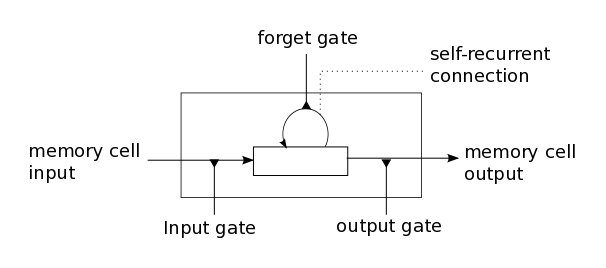
\includegraphics[width=0.7\linewidth]{./figures/lstm_memorycell}
  \caption{LSTM 模型}\label{fig:lstm}
\end{figure}


GRU 可以看成是 LSTM 的变种,GRU 把 LSTM中的 遗忘门和输入门用更新门来替代。 把 cell state 和隐状态 $h_t$ 进行合并,在计算当前时刻新信息的方法和 LSTM 有所不同。 下图是GRU更新 $h_t$ 的过程\cite{DBLP:journals/corr/Pezeshki15}, 具体定义如下:
\begin{itemize}
\item 更新门 $z_t$: 定义保存多少以前的信息:$z_t = \sigma ( W^z x_t+ U^z h_{t-1}  )$

\item 重置门 $r_t$: 决定保留多少输入信息:$r_t = \sigma(W^r x_t  + U^r h_{t-1}  )$

\item 节点内部更新值$\tilde h_t $: 其次是计算候选隐藏层(candidate hidden layer) $\tilde h_t$,这个候选隐藏层 和LSTM中的$\tilde c_t$是类似,可以看成是当前时刻的新信息,其中$r_t$用来控制需要 保留多少之前的记忆,如果$r_t$为0,那么$\tilde h_t$只包含当前词的信息:$\tilde h_t  = \tanh (W^h x_t  + U^h(h_{t-1} \odot r_t) )$

\item 隐藏层输出值$h_t$: 最后$z_t$控制需要从前一时刻的隐藏层 $h_{t-1}$ 中遗忘多少信息,需要加入多少当前 时刻的隐藏层信息$\tilde h_t$,最后得到$h_t$,直接得到最后输出的隐藏层信息, 这里与LSTM的区别是GRU 中没有 输出门:$h_t = (1-z_t)\odot \tilde h_t  + z_t \odot h_{t-1}$
\end{itemize}
如果重置门接近0,那么之前的隐藏层信息就会丢弃,允许模型丢弃一些和未来无关 的信息;更新门 控制当前时刻的隐藏层输出$h_t$需要保留多少之前的隐藏层信息, 若$z_t$接近1相当于我们之前把之前的隐藏层信息拷贝到当前时刻,可以学习长距离依赖。 一般来说那些具有短距离依赖的单元重置门比较活跃(如果$r_t$ 为1,而$z_t$为$0$ 那么相当于变成了一个标准的RNN,能处理短距离依赖),具有长距离依赖的单元更新门比较活跃。

\begin{figure}
  \centering
  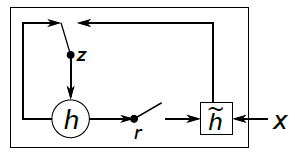
\includegraphics[width=0.5\linewidth]{./figures/gru}
  \caption{GRU模型示意图}\label{fig:gru}
\end{figure}


\subsection{词表分解方案}
通过对基于词表分解的循环神经网络语言模型的探究,我们发现这一类的方法一般都有一些针对词表分解组织结构管理的辅助技术,主要有两种:1)词表分解初始化算法,2)词表动态交换算法。

首先关于词表分解初始化算法:

对于词表分解这一类的方法,他们的核心思想是利用词的结构性,然后先预测词的类别再去具体预测某一个词。对此,词的结构性是一个非常关键的点,词具有什么样的结构性,哪些词可以聚合到一次再合并成一个类,这也叫词的聚类(Clustering),这值得深入的探讨与研究。我们先探究前人在词表分解这些方法中使用的聚类方法。
\begin{itemize}
  \item 随机打乱(Random Shuffle):即随机把词的顺序打乱再划分到一些类别中。
  \item 词频划分(Frequency Binning):先统计语料中每个词出现的频率,再把词按词频大小排序,最后把词按词频大小等距切割成多块,每块中的词具有相近的词频大小。这种方法认为,词的结构性表现在词频中,频率相同或相近的词具备相近的特性。有一些基于词表分解的方法是用该聚类方法的,如\cite{DBLP:conf/nips/MikolovSCCD13,DBLP:conf/acl/ChenGA16}。
  \item 布朗聚类(Brown Clustering):它是一种自底向上的层次聚类算法,基于n-gram模型和马尔科夫链模型(Markov Model);布朗聚类是一种硬聚类,每一个词都在且只在唯一的一个类中。由于布朗聚类的原理本身就通过训练一个语言模型来优化词的结构关系,于是该方法能从一定程度上能从词义的角度将词聚类,其原理如图\ref{fig:brown_cluster}。
\end{itemize}
\begin{figure}[!ht]
  \centering
  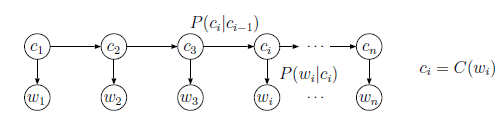
\includegraphics[width=0.65\columnwidth]{./figures/brown_clustering.png}
  \caption{布朗聚类的结构}
  \label{fig:brown_cluster}
\end{figure}

其次关于词表动态交换算法:
\begin{figure}
  \centering
  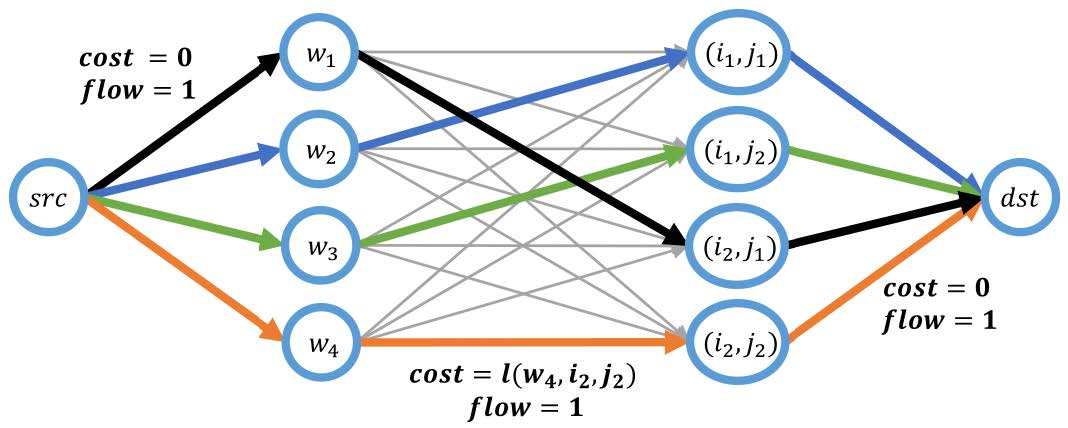
\includegraphics[width=0.65\columnwidth]{./figures/mcmf.jpg}
  \caption{将类别中的词交换问题转化为最小代价最大流问题}
  \label{fig:mcmf}
\end{figure}
前面讲述了用词聚类方法预先将词划分到某些类别中,但这种方法是预训练的,也就是与当前的目标不可见的,那么通过该方法把词聚类并不一定适合模型,也就是说模型的学习过程不能全依赖预先得到的词结构表示。于是就需要一个词表交换算法(Class Exchange Algorithm),在模型的训练过程中将词的类别进行调换以更适用于该模型。LightRNN是典型的使用该思想的模型,它在训练过程中通过计算负对数似然(Negative Logarithm Likelihood, NLL)得到每个词赋给每个类的损失,然后需要找到一种方法让所有词都合理的赋给一个类并使得所有的损失加起来最小。这个问题可以被看作为最小代价最大流(Minimum Cost Maximum Flow, MCMF)的问题或者被看作为分配问题(Assignment Problem),见图\ref{fig:mcmf}。对此,我们需要开发出有效的算法进行更好的词交换。

\subsection{词表分解表示的建模方法研究}
我们在第\ref{sec:hsm}章节中详细介绍了词表分解中cHSM这一类的方法,以及属于这一类方法三种此类组织结构模型。通过分析,我们发现这三种结构虽然其Softmax结构大相径庭,但是他们之间有一点是相同的,就是各自的Softmax预测都是建立在一个隐层状态上的。虽然这个隐层状态所依赖的信息量相对来说比较充分,如当前输入词的信息、所有当前词的历史词的信息,但是cHSM要预测的有词所属的类以及类里面的词两部分,这两部分分别是在两个预测空间里搜索出正确答案。两个预测空间是不一致的,但是他们预测的依赖却是相同的,这可能会存在一些问题。针对这些问题,我们会继续研究挖掘,通过阅读相关的文献,关注相关的最前沿的研究成果,想出一些可能的解决方法,并开始做一些实验去验证与实践。



\section{下一阶段工作计划}

\subsection{时间安排}
\begin{tabular}{r|l}
  % after \\: \hline or \cline{col1-col2} \cline{col3-col4} ...
  2018年5月——2018年7月 & 调研目前前沿的基于词表分解的语言模型 \\
  2018年7月——2018年9月 & 调研并优化基于词表分解循环神经网络 \\
  2018年9月——2018年10月 & 调研并优化词表分解方案 \\
  2018年10月——2018年11月 & 代码实现设计的方法 \\
  2018年11月——2018年12月 & 补充完整实验验证,统计分析实验结果 \\
  2018年12月——2019年1月 & 整理资料和论文撰写
\end{tabular}

\subsection{存在的问题}
\begin{itemize}
  \item 基于GPU的编程增加了coding难度
  \item 计算资源的匮乏使得实验进行缓慢
  \item 数据量极大,建模实验周期长
  \item 一些前沿的方法还没有公开其代码实现
  \item 基础模型采用RNN,当神经模型变得复杂时,建模过程变的不可解释,这对寻找提升模型方法增大了难度
\end{itemize}

\section{总结与展望}
本文首先讲述了论文选题的背景知识和研究意义,介绍了语言模型的背景知识以及对语言模型进行深入研究的重要意义。然后本文介绍了国内外研究现状和发展动态,简要概述了语言模型的一发展历史,从一开始基于统计的N-gram 语言模型,到深度学习被提出以来神经网络模型应用于语言模型使得语言模型的性能得到飞跃的提升,尤其是循环神经网络的引入,这触发了将循环神经网络应用于自然语言处理领域这一热潮。紧接着本文详细的介绍了研究目标和研究内容,从理论上分析循环神经网络语言模型的缺点,分析为何词表过大会带来灾难性的问题,并且详细的介绍了针对这个问题近几年学术界提出的新模型和新方法,本文把这些方法分成三大类,并对每一类方法都进行详细的阐述其原理,并解释为何这些方法能从一定角度上缓解词表过大的问题。再而本文简要的介绍了需要解决的问题和其对应研究路线,对于基于词表分解这一类的模型,本文提出三个重点研究方向,即词聚类方法、词表交换算法和词表分解的建模方式,并尝试从中发掘可以优化的点。

通过阅读大量的关于语言模型的文献,能够对现有的方法都有了一定的了解。下一步,我们将对这些方法进行总结与归纳,发现其中的一些问题,并尝试进行优化。尤其是词表分解这一类的方法,我们可以尝试去做一些优化。针对词表分解这一类的方法,我们已经酝酿了一些初步的想法,下一步是要将想法实践出来,通过实验去验证这些想法,并在这个过程中再去分析和总结,再优化我们的想法。最后,本文列出了具有针对性且详细的研究计划。
\newpage
\addcontentsline{toc}{section}{参考文献}
\bibliography{bibs}

\end{document}
